\documentclass[aspectratio=1610]{beamer}
\hypersetup{
        unicode=true,
        linkcolor=blue,
        anchorcolor=blue,
        citecolor=green,
        filecolor=black,
        urlcolor=blue
    }

%%%%% PACKAGES HERE
%% \usepackage{}
\usepackage{amsmath}
\usepackage{amssymb}
\usepackage{listings}
\usepackage[cache=false]{minted}
\usepackage{textcomp}
\usepackage{xcolor}
\usepackage{tikz}
\usetikzlibrary{positioning,calc}
\usepackage{graphicx}
\usepackage{hyperref}
\usepackage{listings}
\usepackage{fontawesome}
\usepackage[english]{babel}

\setlength{\parskip}{1em}

\usepackage[backend=biber, style=numeric]{biblatex} 
\addbibresource{references.bib}

%%%%%%%%%%%%%%%%%%%%%%%%%%%%%%%%%%%
%% DO NOT CHANGE

\usetheme{default}
\useinnertheme{circles}
\useoutertheme{infolines}
\usefonttheme{serif}

\usepackage{etoolbox}

%% T for navigation symbols
%%\setbeamertemplate{navigation symbols}{}

%% T for header
%% \setbeamertemplate{headline}{%
%%   \leavevmode%
%%   \ifdefempty{\insertsubsectionhead}{
%%     \begin{beamercolorbox}[wd=0.99\paperwidth,ht=2.25ex,dp=1ex,center]{section in head/foot}%
%%       % \hbox to .5\paperwidth{\hfil\insertsectionhead\hfil}
%%       \insertsectionhead
%%     \end{beamercolorbox}%
%%   }{
%%     \begin{beamercolorbox}[wd=.44\paperwidth,ht=2.25ex,dp=1ex,right]{section in head/foot}%
%%       % \hbox to .5\paperwidth{\hfil\insertsectionhead\hfil}
%%       \insertsectionhead
%%     \end{beamercolorbox}%
%%     \begin{beamercolorbox}[wd=.1\paperwidth,ht=2.25ex,dp=1ex,center]{section in head/foot}%
%%       % \hbox to .5\paperwidth{\hfil\insertsectionhead\hfil}
%%       -
%%     \end{beamercolorbox}%
%%     \begin{beamercolorbox}[wd=.44\paperwidth,ht=2.25ex,dp=1ex,left]{subsection in head/foot}%
%%       % \hbox to .5\paperwidth{\hfil\insertsubsectionhead\hfil}
%%       \insertsubsectionhead
%%     \end{beamercolorbox}
%%   }%
%% }

%% T for frame title
\setbeamertemplate{frametitle}{%
  \usebeamerfont{frametitle}\insertframetitle\strut%
  \vskip-0\baselineskip%
  \leaders\vrule width .95\paperwidth\vskip1pt%
  \vskip0pt%
  \nointerlineskip
}

%% T for footer
\setbeamercolor{footlinecolor}{fg=cyan,bg=green}
\setbeamercolor{author in head/foot}{fg=blue}

\setbeamertemplate{footline}{%
  \leavevmode%
  \hbox{%
  \begin{beamercolorbox}[wd=.26\paperwidth,ht=2.25ex,dp=1ex,left]{author in head/foot}%
    \hspace*{2ex}\usebeamerfont{author in head/foot} SIMIS
  \end{beamercolorbox}%
  \begin{beamercolorbox}[wd=.50\paperwidth,ht=2.25ex,dp=1ex,center]{author in head/foot}%
    \usebeamerfont{title in head/foot} Improving the Minkowski Constant Using the Exponent of Decay
  \end{beamercolorbox}%
  \begin{beamercolorbox}[wd=.24\paperwidth,ht=2.25ex,dp=1ex,right]{date in head/foot}%
    \usebeamerfont{date in head/foot}
    \insertshortdate{}\hspace*{1em}  % date
    \insertframenumber/\inserttotalframenumber\hspace*{2ex}
  \end{beamercolorbox}}%
  \vskip0pt%
}
%%%%%%%%%%%%%%%%%%%%%%%%%%%%%%%%%%%%%%%%%%%%%%%%

\begin{document}

%Brief Introduction about contents, overall statement of Major results.%
\section{Introduction}
\begin{frame}
    \frametitle{Introduction to Multidimensional Diophantine Approximation}
    %Say: In a single dimension, Diophantine approximation is a well-understood topic and the first few of our lectures in Analysis & Number Theory are all about working in one dimension.
    %     However, what happens when we wish to approximate multiple irrational numbers at once?
    
    Approximating an irrational vector $\boldsymbol{\alpha} \in \mathbb{R}^d$ with integer vectors:
    %Say: There are actually two ways of approximating our irrational vector alpha.

    \textbf{Simultaneous Approximation (SA)}
    seeks to find approximation vectors $(q,\mathbf{p}) \in \mathbb{Z}^+ \times \mathbb{Z}^d$ which minimize $ || q\boldsymbol{\alpha} - \mathbf{p} ||_2$
    %Say: In other words, we're approximating all coordinates of alpha by rationals with the same denominator q.
    %Say: Here ||•||2 denotes the Euclidean norm, or the euclidean distance to the origin.
    %     For clarity, we will leave out the subscript from here onwards.

    \textbf{Linear Form Approximation (LF)}
    seeks to find approximation vectors $(\mathbf{q},p) \in \mathbb{Z}^d \times \mathbb{Z} \setminus \{\textbf{0}\}$ which minimize
    $| \mathbf{q} \cdot \boldsymbol{\alpha} - p | = |q_1\alpha_1 + ... + q_n\alpha_n - p|$.
    %Say: In other words, we're selecting integers q1, q2, ..., qn to make q1a1 + ... + qnan as close to an integer as possible.
    %Say: As an additional constraint, the coordinates of alpha must all be irrational and linearly independent over Q, since otherwise we can get 0 in LF.

    %Say: Quite trivially one can show that in gboth cases |qa-p| can get arbitrarily close to zero.
    %     Therefore we need more constraints, which is generally chosen to be size of q.
    In this presentation we will mainly be working with two-dimensional LF approximations in the Euclidean norm.
    %     However, our results are easily generalized to an arbitrary dimension and norm, for both SA and LF.
    
    \begin{definition}[Minkowski Constant for LF]
        The smallest constant $c$ such that for any $\boldsymbol{\alpha}$ there exist infinitely many approximations $(\mathbf{q},p) \in \mathbb{Z}^3$
        which satisfy $| \mathbf{q} \cdot \boldsymbol{\alpha} - p | < \dfrac{1}{c||\textbf{q}||^2}$.
    \end{definition}
    %Say: In other words, "a large c implies that we will find very good approximations".

\end{frame}

\begin{frame}
    \frametitle{Geometrical Interpretation}
    For positive constants $c_l$, $c_s$, define the following sets:
    \[S_l := \left\{(x_1,x_2, y)\in \mathbb{R}^3:\ |\alpha_1x_1 + \alpha_2x_2-y| < \frac{1}{c_l||(x_1,x_2)||^2}\right\}\]
    \[S_s := \left\{(y_1, y_2, x)\in \mathbb{R}^3: \ ||(\alpha_1x - y_1, \alpha_2x-y_2)|| < \frac{1}{c_s\sqrt{|x|}}\right\}\]
    %Say: Notice that the definition of Minkowski Constant is equivalent to saying that for any vector alpha, Sl (or Ss) contains infinitely many lattice points.
    %     This definition allows us to convert the number-theoretical problem into geometry, and we shall utilize the Minkowski Convex Body Theorem to find infinitely many lattice points within the set.
    \begin{theorem}[Minkowski]
        Let $A \subset \mathbb{R}^d$ be a measurable set which is convex and symmetric about the origin. If $\mathrm{vol}(A)>2^d$, then $A$ contains a nonzero point in $\mathbb{Z}^d$.
    \end{theorem}
    %Say: We will discuss how this theorem is to be applied later in this presentation.

    %Say: Now we present the notion of duality between linear form and simultaneous approximations.
\end{frame}

\subsection{1.2 Duality between SA and LF in 2-d Space}
\begin{frame}
    \centering
    \begin{tikzpicture}[every node/.style={inner sep=0pt}]
        % Nodes
        \node (LF) {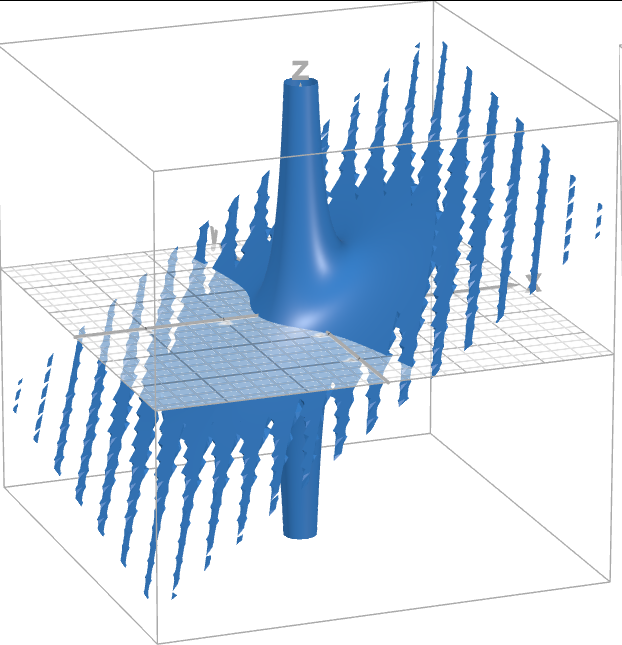
\includegraphics[width=0.26\textwidth]{LF.png}};
            \node[yshift=-48pt] at (LF) {$S_l$};
        \node[right=4cm of LF] (STD) {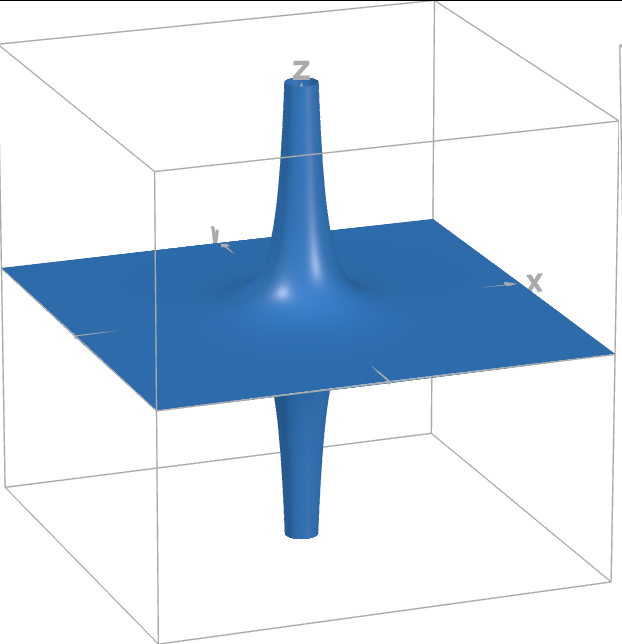
\includegraphics[width=0.26\textwidth]{STANDARD.png}};
            \node[yshift=-48pt] at (STD) {$S$};
        \node[below=0.5cm of STD] (SA) {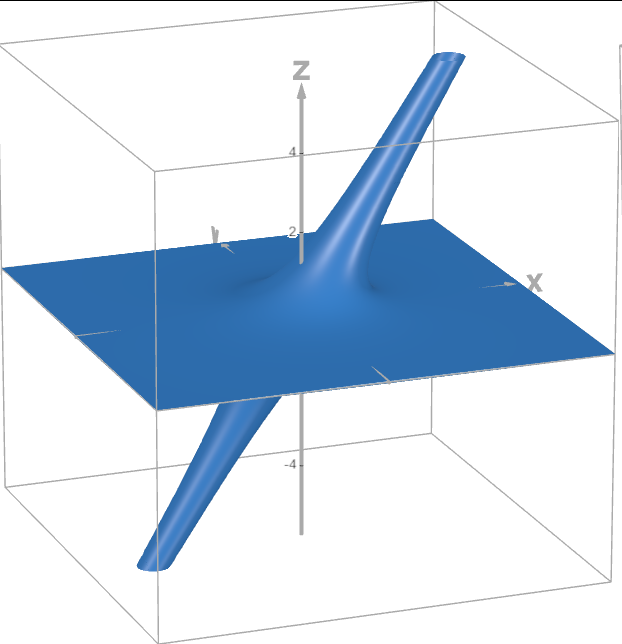
\includegraphics[width=0.26\textwidth]{SA.png}};
            \node[yshift=-48pt] at (SA) {$S_s$};
        \node[below=0.5cm of LF, align=center] (textBL) {
        $\chi=$
        $\displaystyle
        \begin{bmatrix}
            1&&-\alpha_1\\
            &1&-\alpha_2\\
            &&1
        \end{bmatrix}$\quad

        $\chi^\top=$
        $\displaystyle
        \begin{bmatrix}
            1&&\\
            &1&\\
            -\alpha_1&-\alpha_2&1
        \end{bmatrix}$ \\ \\
        \vspace{0.1cm}Taking $S := \left\{(x, y, z):\ ||(x,y)||^2|z|<\frac{1}{k}\right\}$\\
        \vspace{0.1cm}and choosing $c_s^2 = k = c_l$,\\
        we notice $S_s \xrightarrow{\chi} S \xleftarrow{\chi^\top} S_l$
        };

        % Arrows
        \draw[->, thick] (LF) -- node[above, yshift=3pt] {$\chi^\top$} (STD);
        \draw[->, thick] (SA) -- node[right, xshift=3pt] {$\chi$} (STD);
    \end{tikzpicture}
    
\end{frame}
\end{document}
